% !TeX spellcheck = en_GB
\section{Verification}
In this section we present tests performed in order to verify our implementation.

\subsection{Degeneracy Tests}
In the degeneracy tests we verify the behaviour of our simulator with parameters set to 0 values. In all tests the simulator works properly. In particular the following observations can be inferred:
\begin{itemize}
	\item If the number of channel is 0 then the simulation stops immediately because has no sense running a simulation with 0 channels.
	\item If the time slot size is 0 then the simulation doesn't stop and goes to infinite because on instant 0  time slots are continuously triggered.
	\item If the exponential mean is 0 then the simulation doesn't stop and continues to infinite because packets arrive at time 0 continuously.
\end{itemize}

\subsection{Consistency Test}
The consistency test verifies that the system react consistently with the output. In order to test this we perform two tests with the following parameters.
\paragraph{Test 1}
\begin{itemize}
	\item Number of transmitters: 1
	\item Number of channels: 500
	\item Send probability: 1
	\item Mean inter-arrival time: 10s (deterministic)
	\item Time slot size: 5s
\end{itemize}

\paragraph{Test 2}
\begin{itemize}
	\item Number of transmitters: 2
	\item Number of channels: 500
	\item Send probability: 1
	\item Mean inter-arrival time: 20s (deterministic)
	\item Time slot size: 5s
\end{itemize}

\noindent We expect that the result of the two tests are more or less equal because the behaviour of one source transmitting every 10 seconds must be similar to the behaviour of two sources transmitting every 20 seconds. We set the number of channels at 500 in order to neglect the effect of collisions (in any case it is possible that a collision occur, but in the following tests no collisions have been detected).

\noindent The graph in figure \ref{img: consistencyTest1a} and in figure \ref{img: consistencyTest1b} show the results of the tests previously explained. We can see that the behaviour is very similar in both cases and so that the systems works as we expect.

\begin{figure}[htpb]
	\centering
	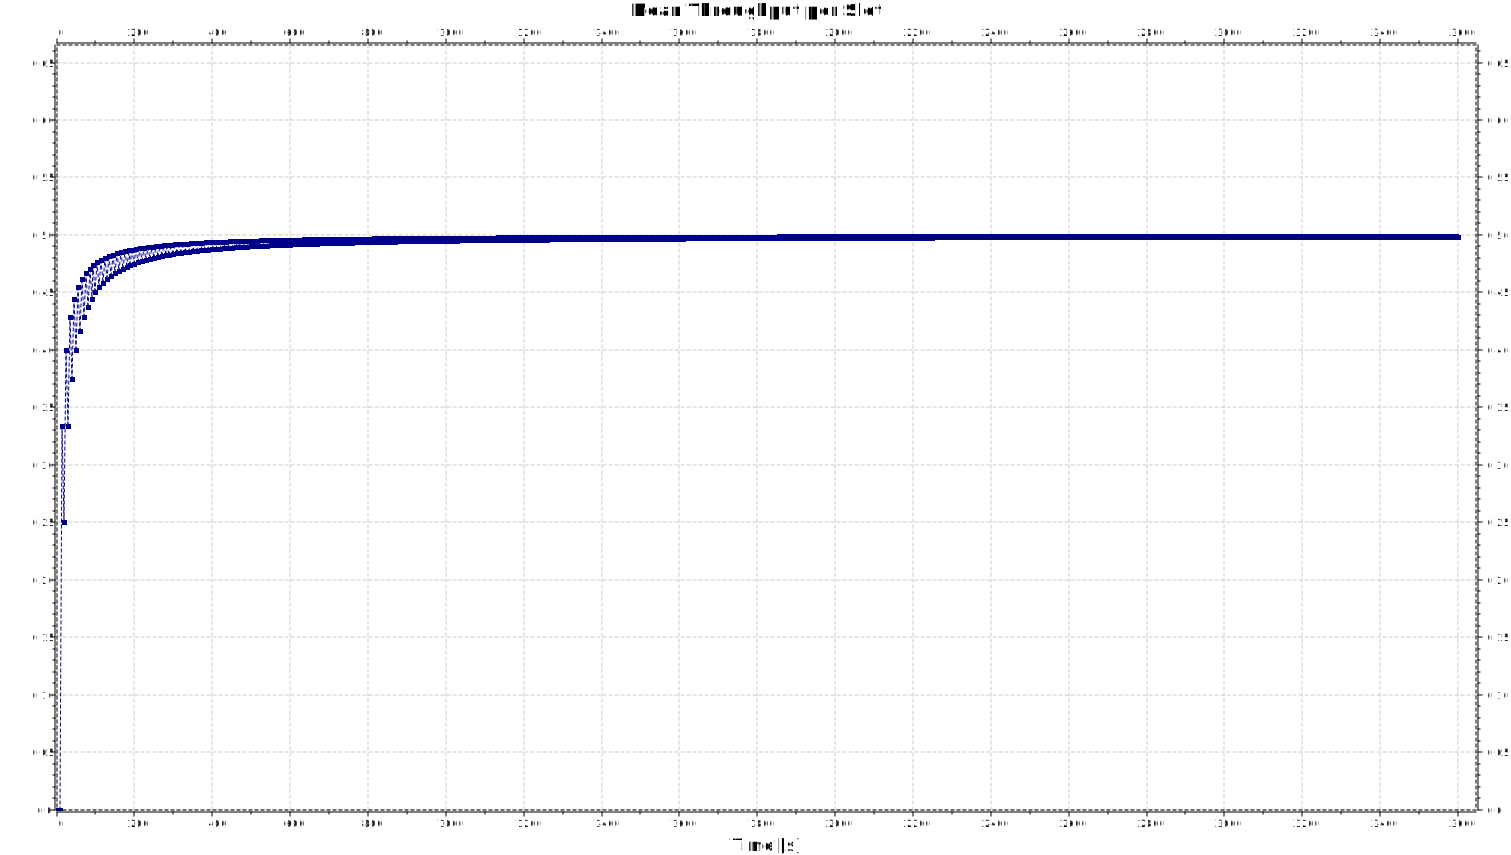
\includegraphics[scale=0.28]{img/ConsistencyTest1a.png}
	\caption{Consistency Test 1}
	\label {img: consistencyTest1a}
\end{figure}

\begin{figure}[htpb]
	\centering
	\includegraphics[scale=0.28]{img/ConsistencyTest1b.png}
	\caption{Consistency Test 2}
	\label {img: consistencyTest1b}
\end{figure}

\noindent The oscillations at the beginning are due to the fact that the mean inter-arrival time is bigger with respect to the time slot size. In fact we can observe that in the second test there are larger oscillations because the difference between the mean inter-arrival time and the time slot size is bigger than the one of the first test.
\subsection{Continuity Test}


\subsection{Test Simulations}
